% !TeX root = ../main.tex

\chapter{YOLOv5 目标检测推理应用开发}

\section{总体流程}

任务 3 完整链路如下：

\begin{lstlisting}[caption={总体流程}]
准备 YOLOv5 代码
  -> 生成权重文件
  -> 导出 onnx 模型
  -> 使用 ATC 转换 OM
  -> 通过 HDC 部署 OM、图片和 Python 程序
  -> 设备端 source CANN 环境变量
  -> Python CLI 读取图片
  -> letterbox 预处理
  -> ais_bench 调用 CANN OM 推理
  -> YOLOv5 NMS 后处理
  -> 绘制检测框
  -> 保存结果图片、txt 和 json
  -> hdc file recv 拉回结果
\end{lstlisting}

CLI 程序入口为：

\begin{lstlisting}[caption={CLI 入口}]
/cann-install/yolov5_cli/main.py
\end{lstlisting}

该程序支持两种后端：

\begin{itemize}
  \item \texttt{ais\_bench}：设备端 OM/NPU 推理。
  \item \texttt{onnxruntime}：PC 端 CPU 冒烟测试，可用于验证预处理和后处理逻辑。
\end{itemize}


\section{准备 YOLOv5 ONNX 模型}

由于本组机器性能不够，所以模型生成和转换部分在云服务器上进行，使用的云服务器提供商为恒源云。
首先在云服务器上克隆YOLOv5源码\hyperref[ref:yolov5]{[14]} ，然后进行训练，生成 .pt 权重文件，接着导出为 ONNX 模型。

\begin{lstlisting}[style=shell, caption={导出 ONNX}]
#clone 源码
git clone https://github.com/ultralytics/yolov5.git
cd yolov5

#环境依赖安装
pip install -r requirements.txt

#训练生成权重文件
python train.py --data coco128.yaml --weights '' --cfg yolov5s.yaml --img 640

#导出 onnx 模型文件
python export.py --weights yolov5s.pt --include onnx --opset 12 --imgsz 640 --dynamic --simplify
\end{lstlisting}

运行完成后即可获得模型文件：\texttt{yolov5s.onnx}

\begin{figure}[H]
  \centering
  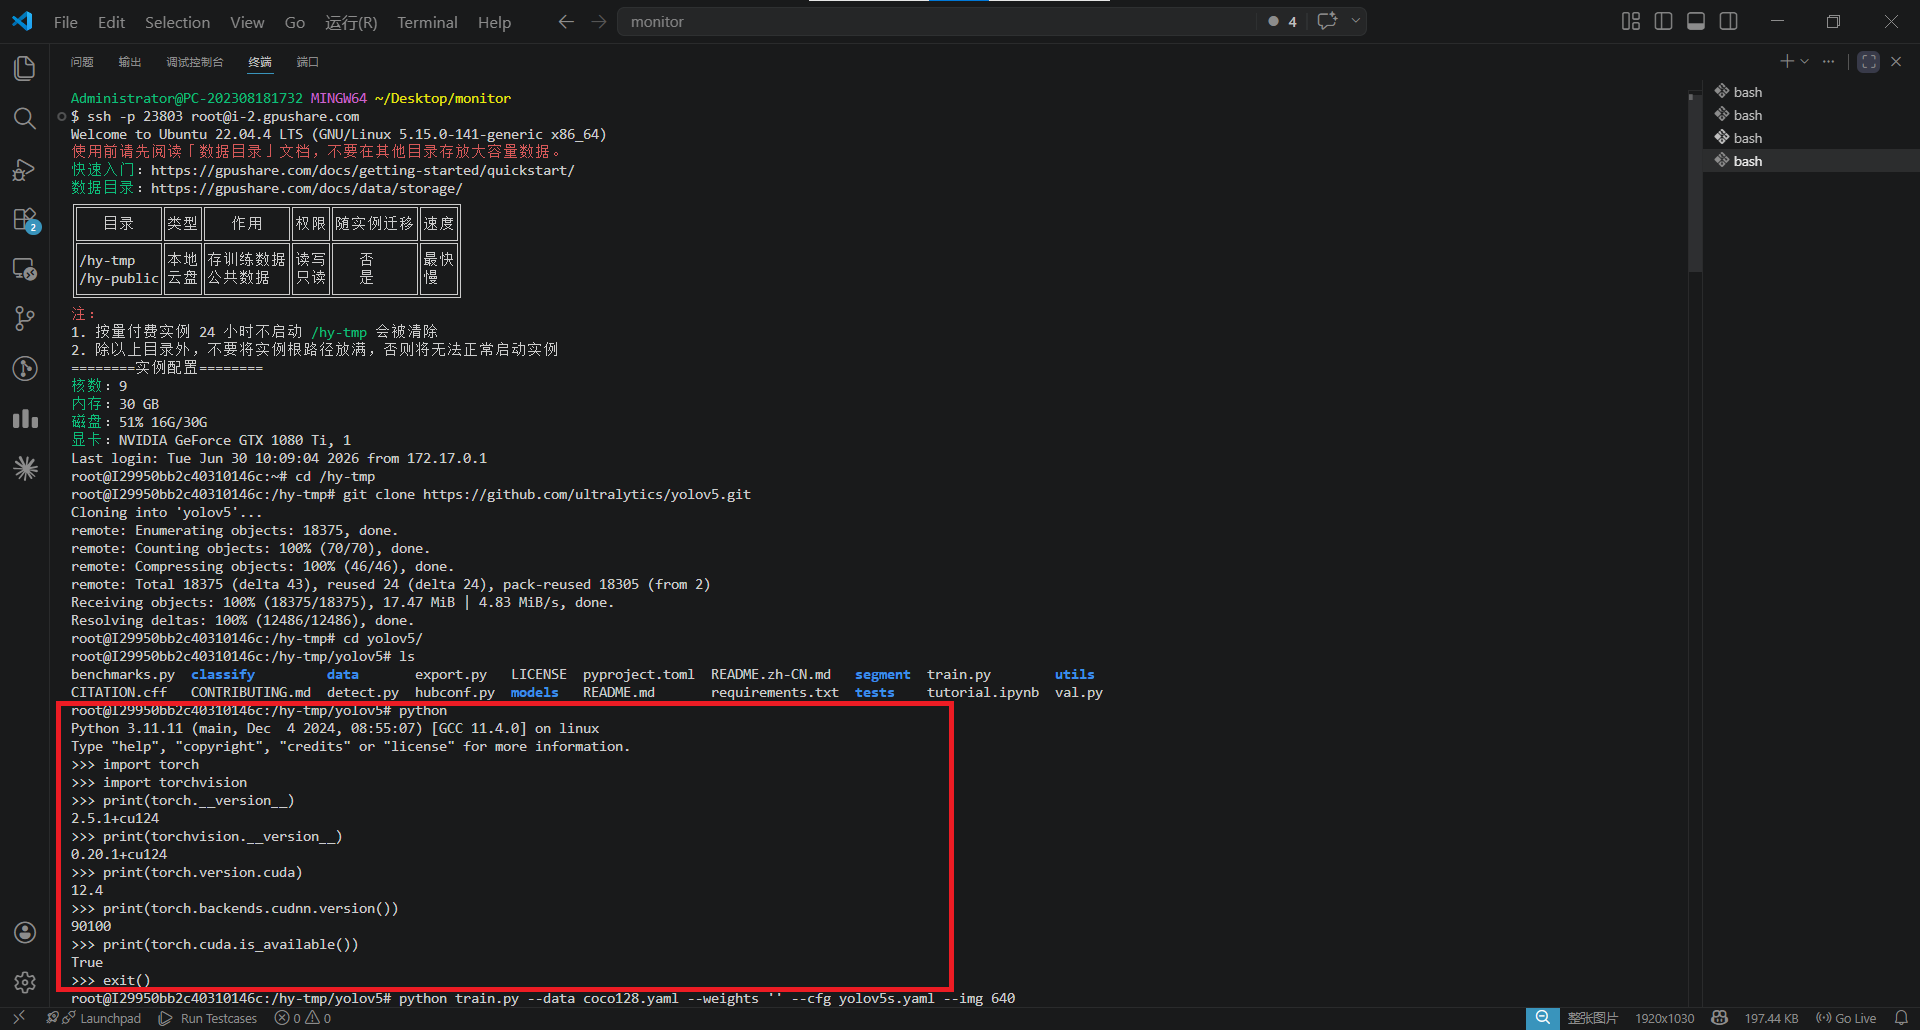
\includegraphics[width=0.8\textwidth]{test_environment.png}
  \caption{验证PyTorch的可用性}
  \label{fig:test_environment}
\end{figure}

\begin{figure}[H]
  \centering
  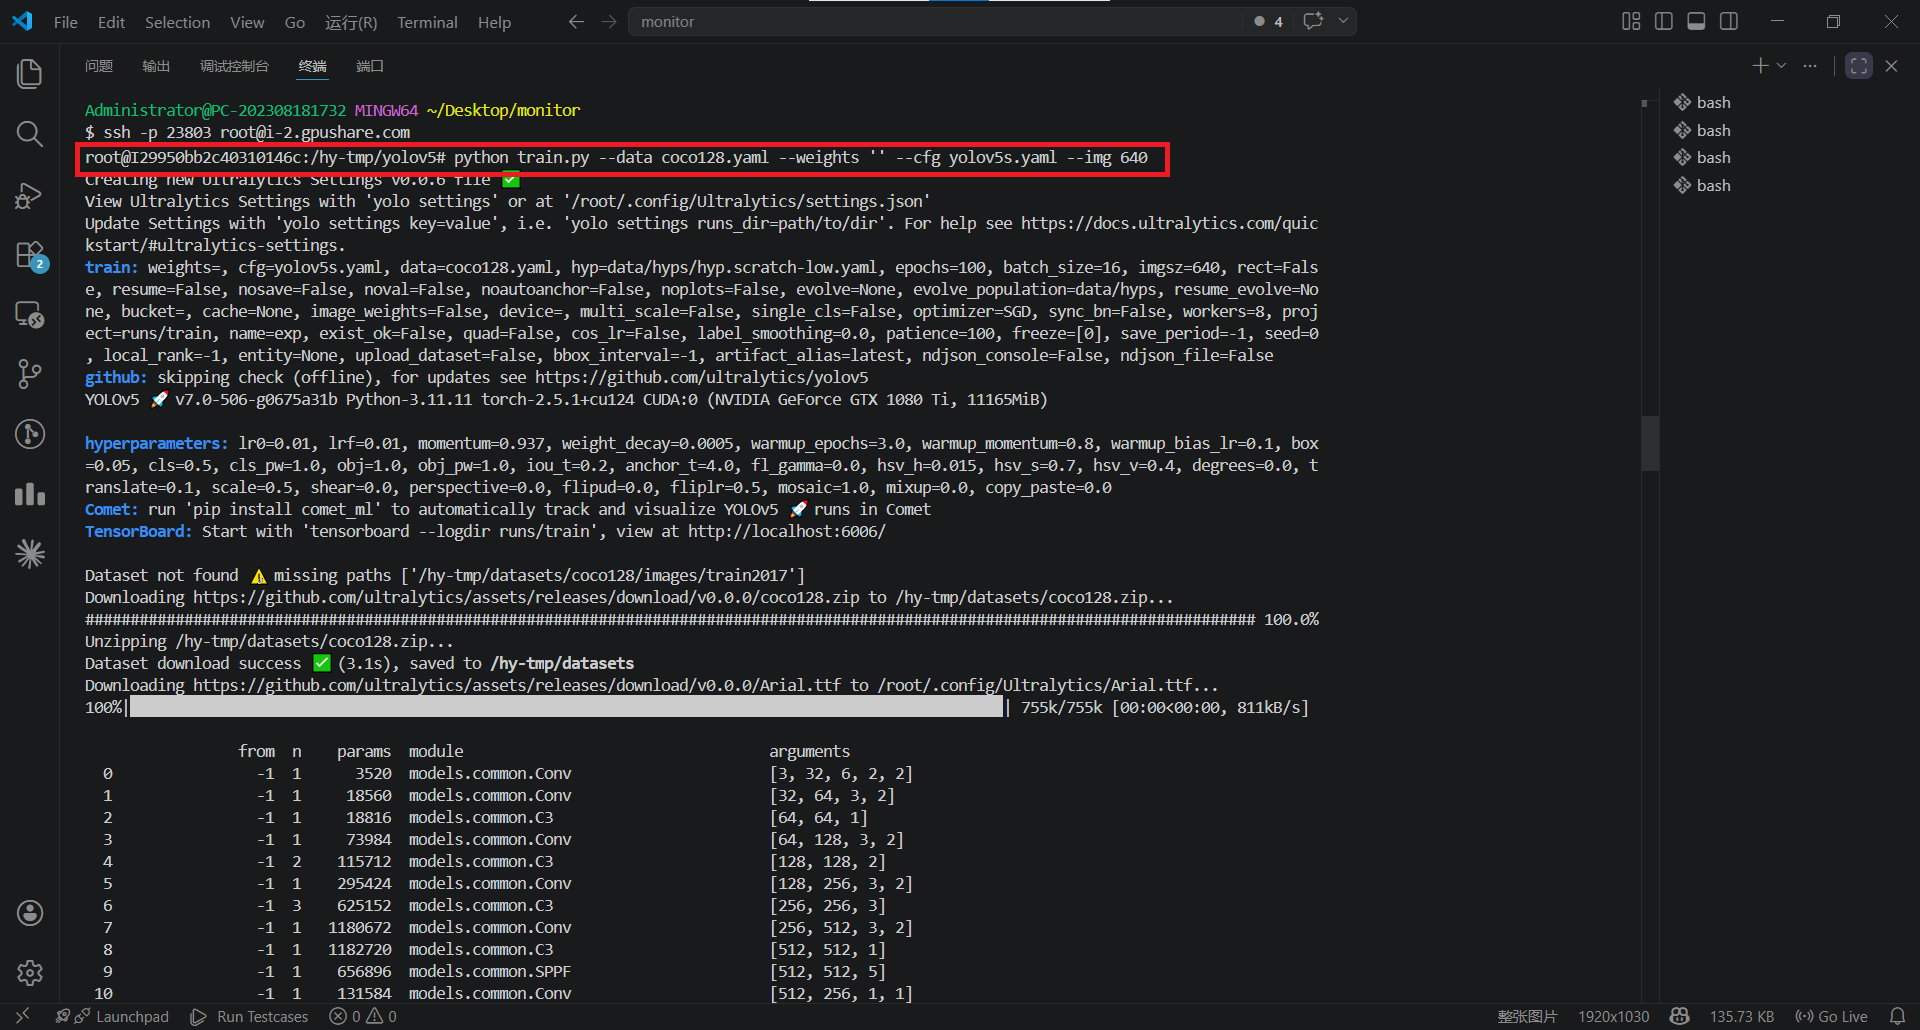
\includegraphics[width=0.8\textwidth]{start_train.png}
  \caption{开始训练}
  \label{fig:start_train}
\end{figure}

\begin{figure}[H]
  \centering
  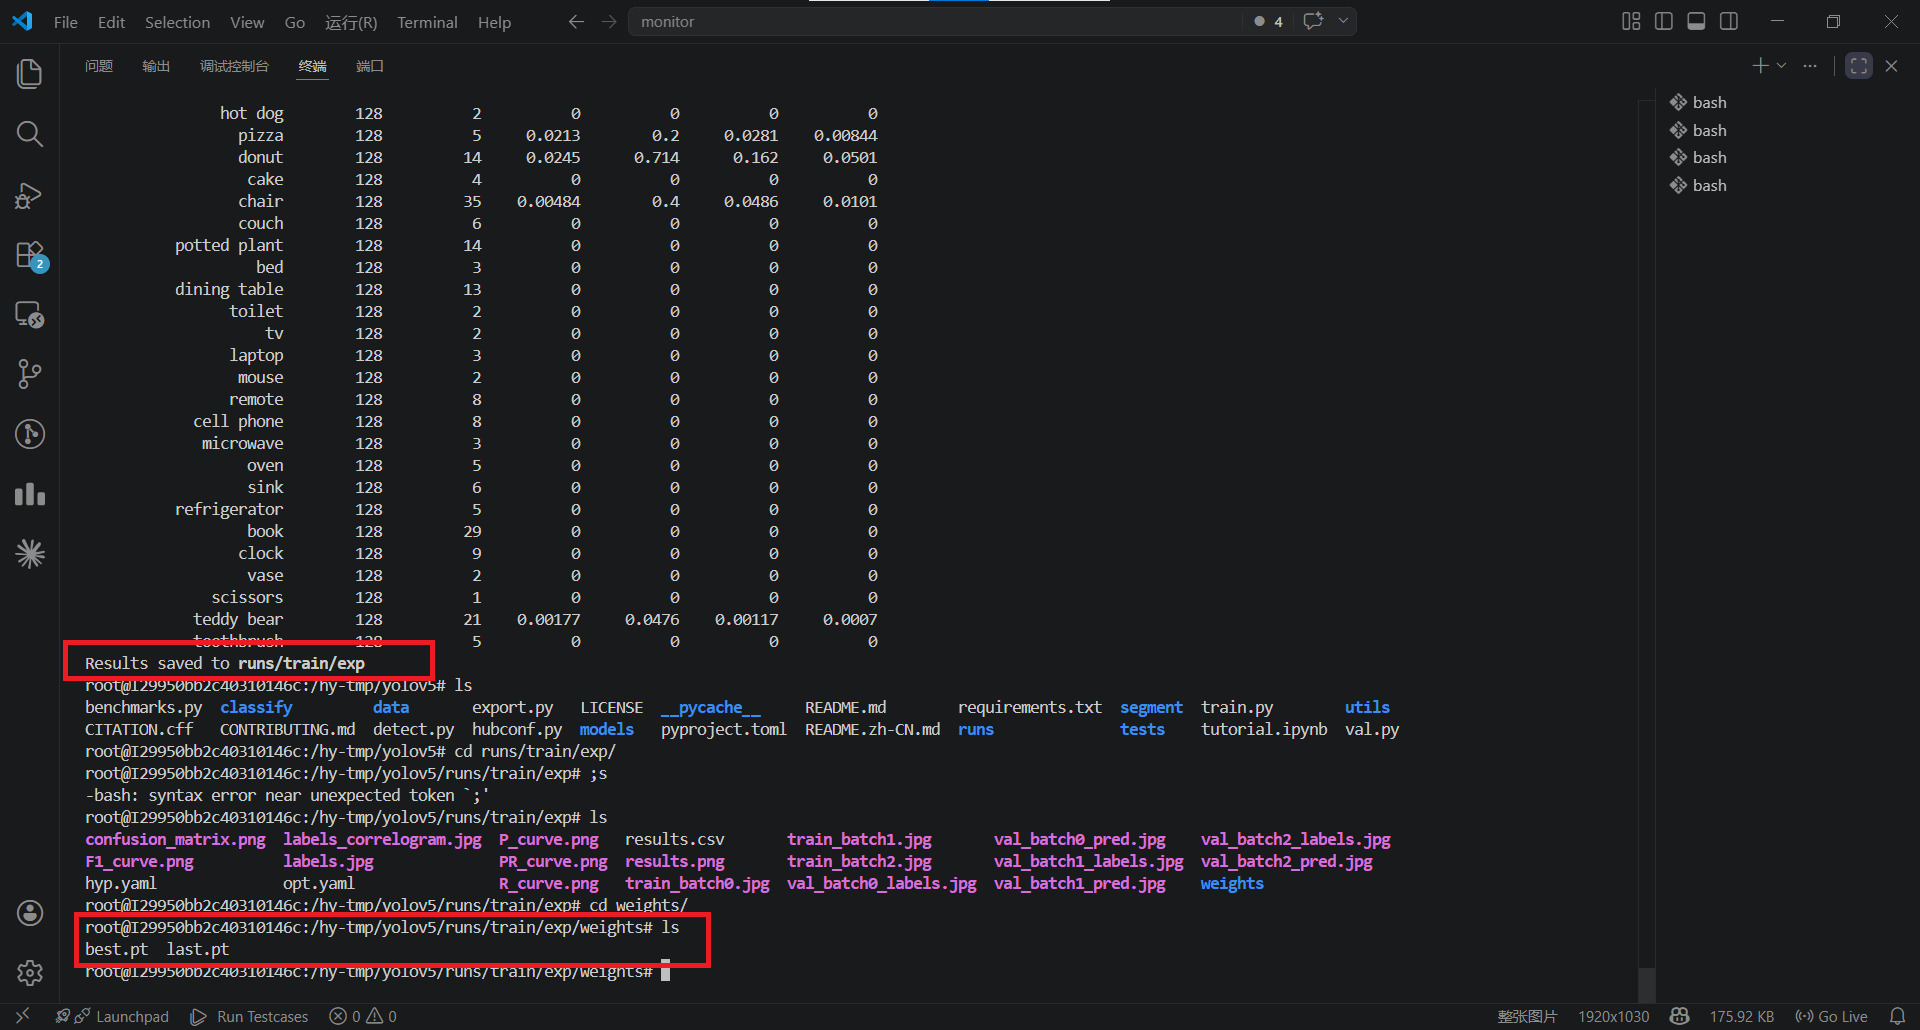
\includegraphics[width=0.8\textwidth]{pt.png}
  \caption{pt 文件获得}
  \label{fig:pt}
\end{figure}

\section{ONNX 转 OM}

\subsection{配置虚拟环境}

首先在云服务器中安装 Anaconda 或者 Miniconda，二选一，本组选择装Anaconda。

\begin{figure}[htbp]
  \centering
  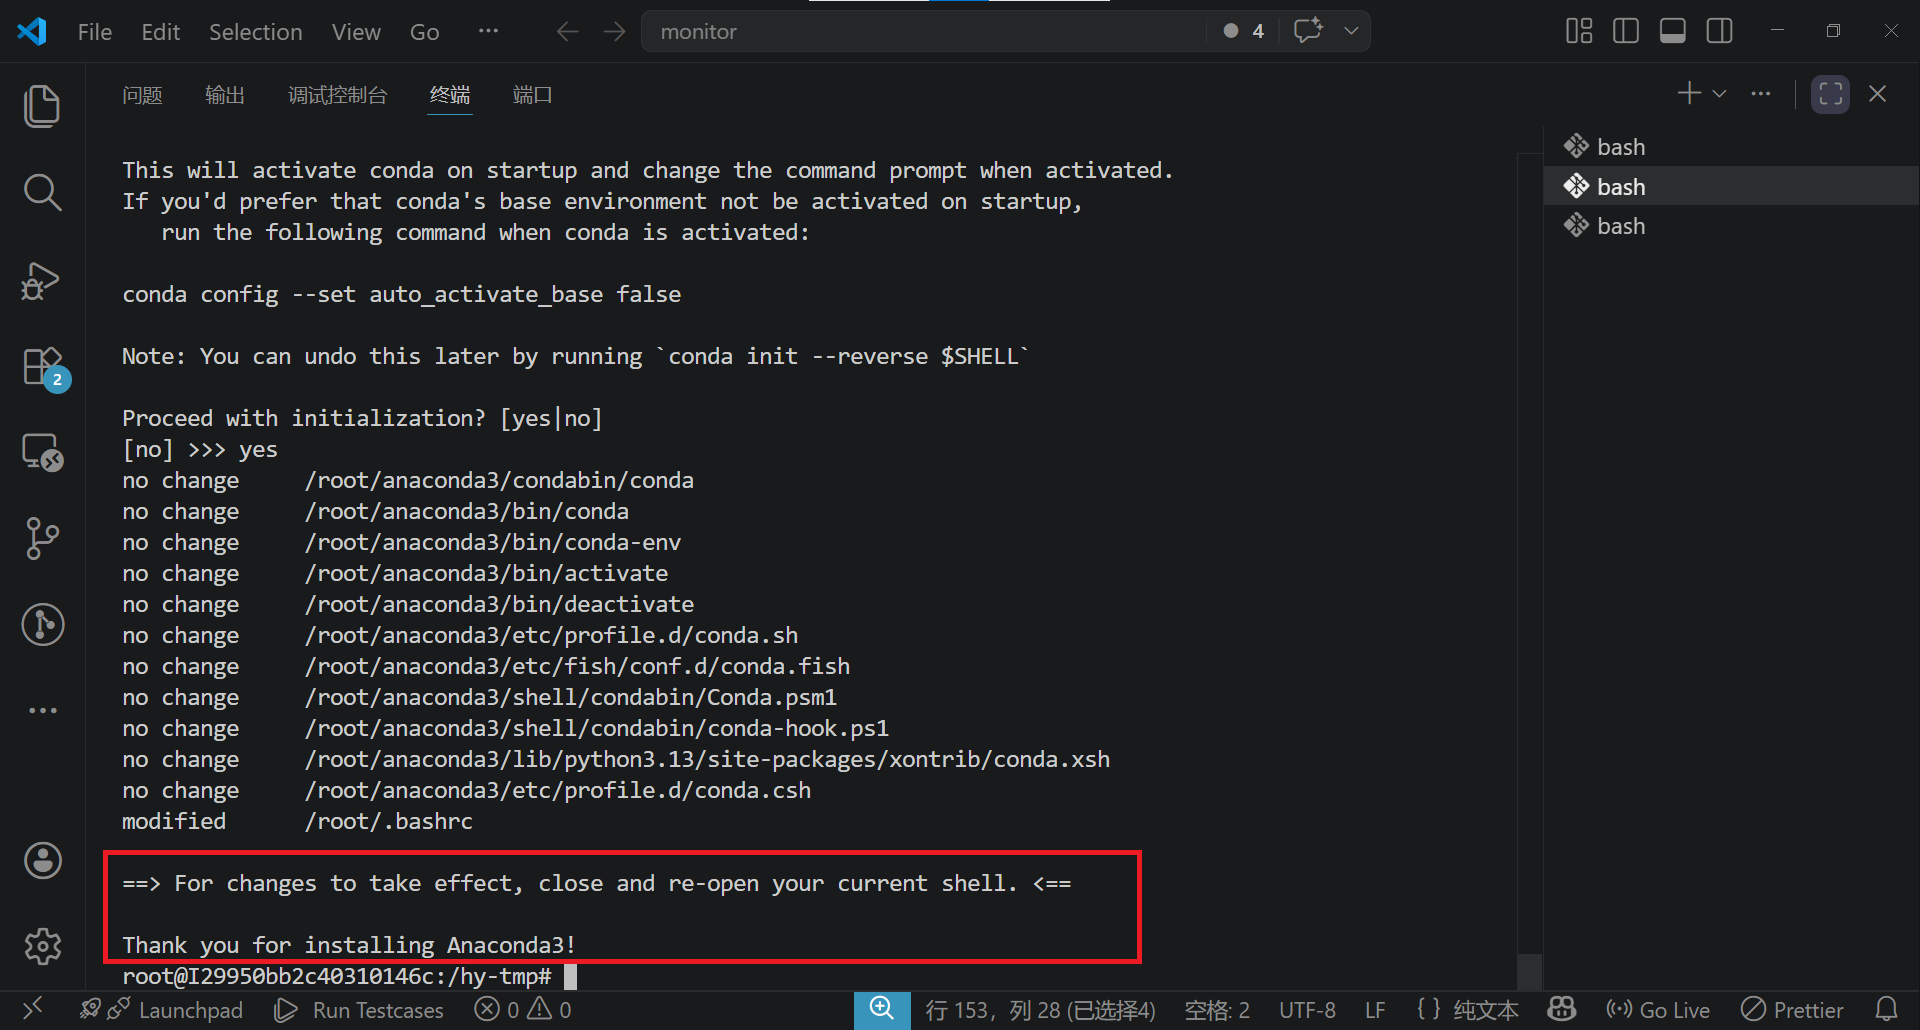
\includegraphics[width=0.8\textwidth]{Anaconda-install.png}
  \caption{Anaconda安装结果}
  \label{fig:Anaconda-install}
\end{figure}

安装完成后，配置虚拟环境：

\begin{lstlisting}[style=shell, caption={创建虚拟环境}, basicstyle=\ttfamily\footnotesize]
#创建环境
conda create -n onnx-to-om python=3.7.5

#激活环境
conda activate onnx-to-om

#进入环境后，安装python依赖
sudo apt-get install -y gcc g++ make cmake zlib1g zlib1g-dev \
  openssl libsqlite3-dev libssl-dev libffi-dev libbz2-dev \
  libxslt1-dev unzip pciutils net-tools libblas-dev gfortran libblas3

#安装python库
pip install attrs -i https://pypi.tuna.tsinghua.edu.cn/simple
pip install numpy -i https://pypi.tuna.tsinghua.edu.cn/simple
pip install decorator -i https://pypi.tuna.tsinghua.edu.cn/simple
pip install sympy -i https://pypi.tuna.tsinghua.edu.cn/simple
pip install cffi -i https://pypi.tuna.tsinghua.edu.cn/simple
pip install pyyaml -i https://pypi.tuna.tsinghua.edu.cn/simple
pip install pathlib2 -i https://pypi.tuna.tsinghua.edu.cn/simple
pip install psutil -i https://pypi.tuna.tsinghua.edu.cn/simple
pip install protobuf -i https://pypi.tuna.tsinghua.edu.cn/simple
pip install scipy -i https://pypi.tuna.tsinghua.edu.cn/simple
pip install requests -i https://pypi.tuna.tsinghua.edu.cn/simple
pip install absl-py -i https://pypi.tuna.tsinghua.edu.cn/simple
\end{lstlisting}

\begin{figure}[htbp]
  \centering
  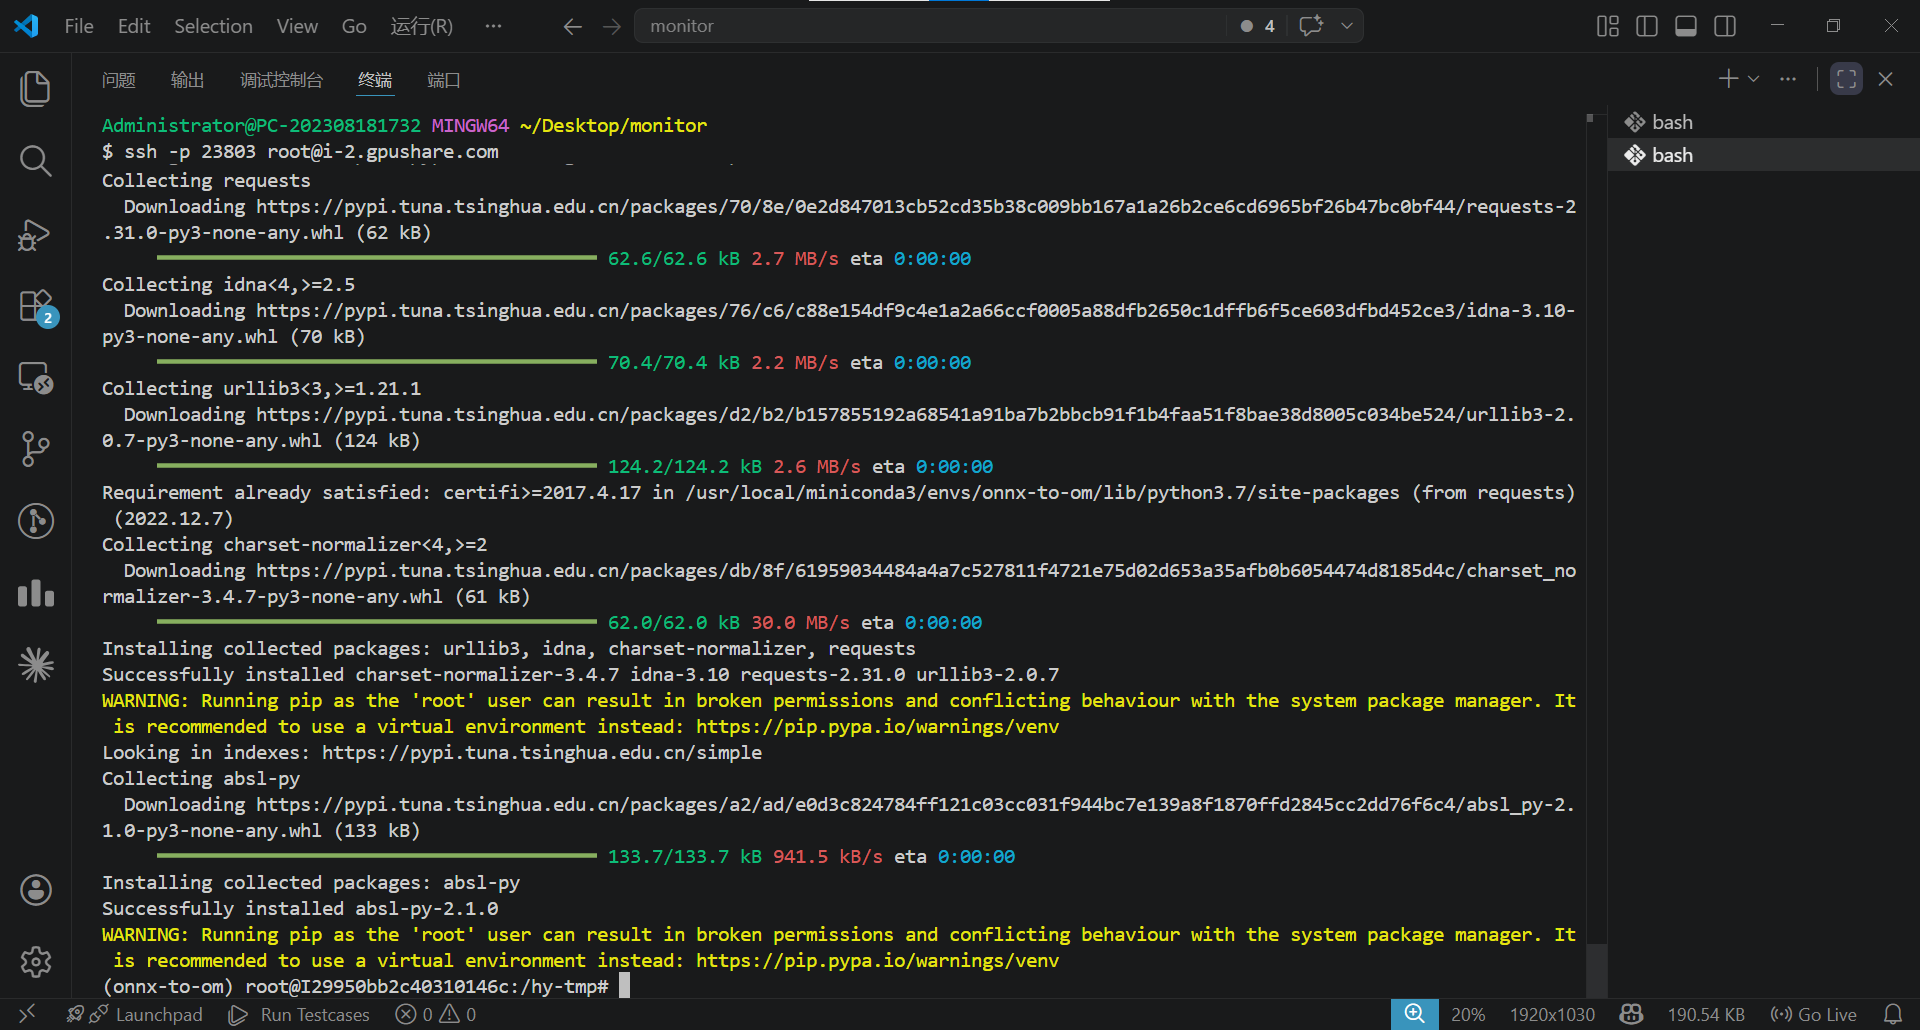
\includegraphics[width=0.8\textwidth]{virtual-environemt.png}
  \caption{虚拟环境安装与配置}
  \label{fig:virtual-environemt}
\end{figure}

\subsection{安装 CANN-toolkit}

接下来下载所需 CANN 文件，由于在云服务器上只是转换文件，所以只需要 CANN\_toolkit 一个软件包，下载 8.2.RC1 版本的 CANN\hyperref[ref:cann-download]{[15]}。

\begin{figure}[htbp]
  \centering
  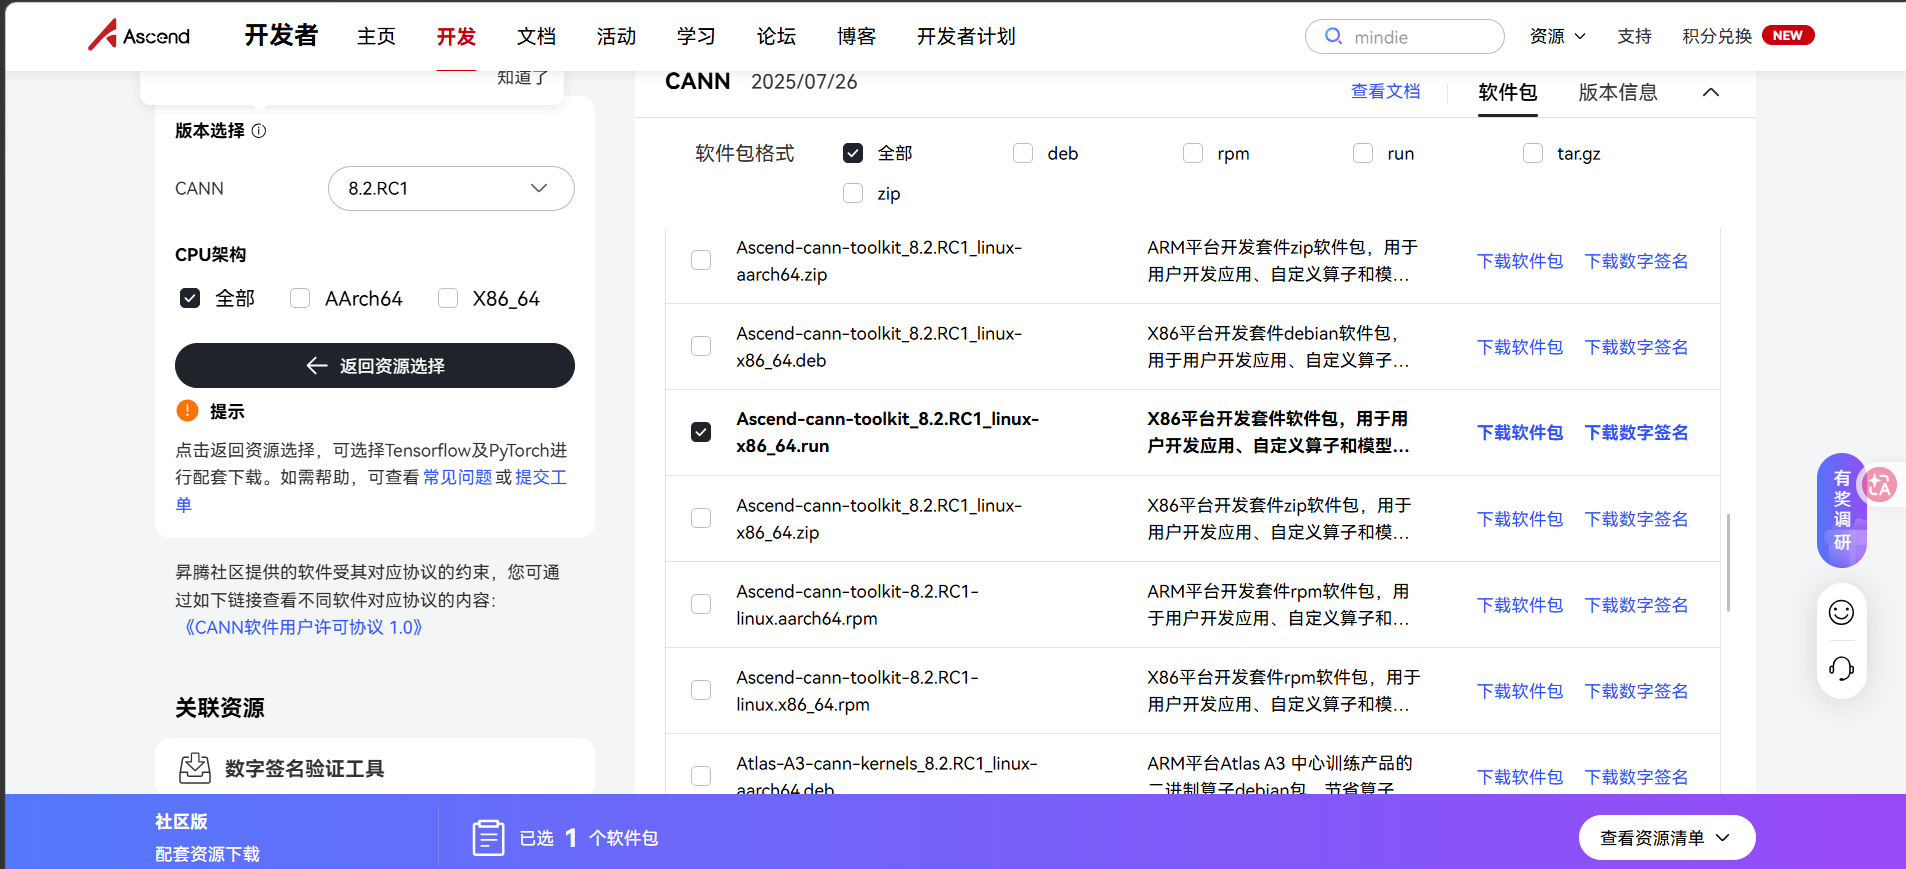
\includegraphics[width=0.8\textwidth]{docx_image2.png}
  \caption{CANN 下载页面}
  \label{fig:cann-download}
\end{figure}

下载完成后，创建个 CANN 文件夹，用于存放文件。

\begin{lstlisting}[style=shell, caption={安装 CANN-toolkit}]
#进入文件夹
cd CANN

# 添加执行权限
sudo chmod +x Ascend-cann-toolkit_8.2.RC1.alpha003_linux-x86_64.run

# 检查一下文件
./Ascend-cann-toolkit_8.2.RC1.alpha003_linux-x86_64.run --check

# 安装文件
./Ascend-cann-toolkit_8.2.RC1.alpha003_linux-x86_64.run --install

\end{lstlisting}

\subsection{配置环境变量}

在脚本末尾添加下面语句，\texttt{CANN\_INSTALL\_PATH} 是 CANN 软件安装目录。

\begin{lstlisting}[style=shell, caption={配置 CANN 环境变量}]
#编辑bashrc
gedit ~/.bashrc

# 例如
source CANN_INSTALL_PATH/ascend-toolkit/set_env.sh
export LD_LIBRARY_PATH=CANN_INSTALL_PATH/ascend-toolkit/latest/x86_64-linux/devlib/:$LD_LIBRARY_PATH

# 实际
source /home/om/Ascend/ascend-toolkit/set_env.sh
export LD_LIBRARY_PATH=/home/om/Ascend/ascend-toolkit/latest/x86_64-linux/devlib/:$LD_LIBRARY_PATH

# 更新一下脚本
source ~/.bashrc
\end{lstlisting}

\begin{figure}[H]
  \centering
  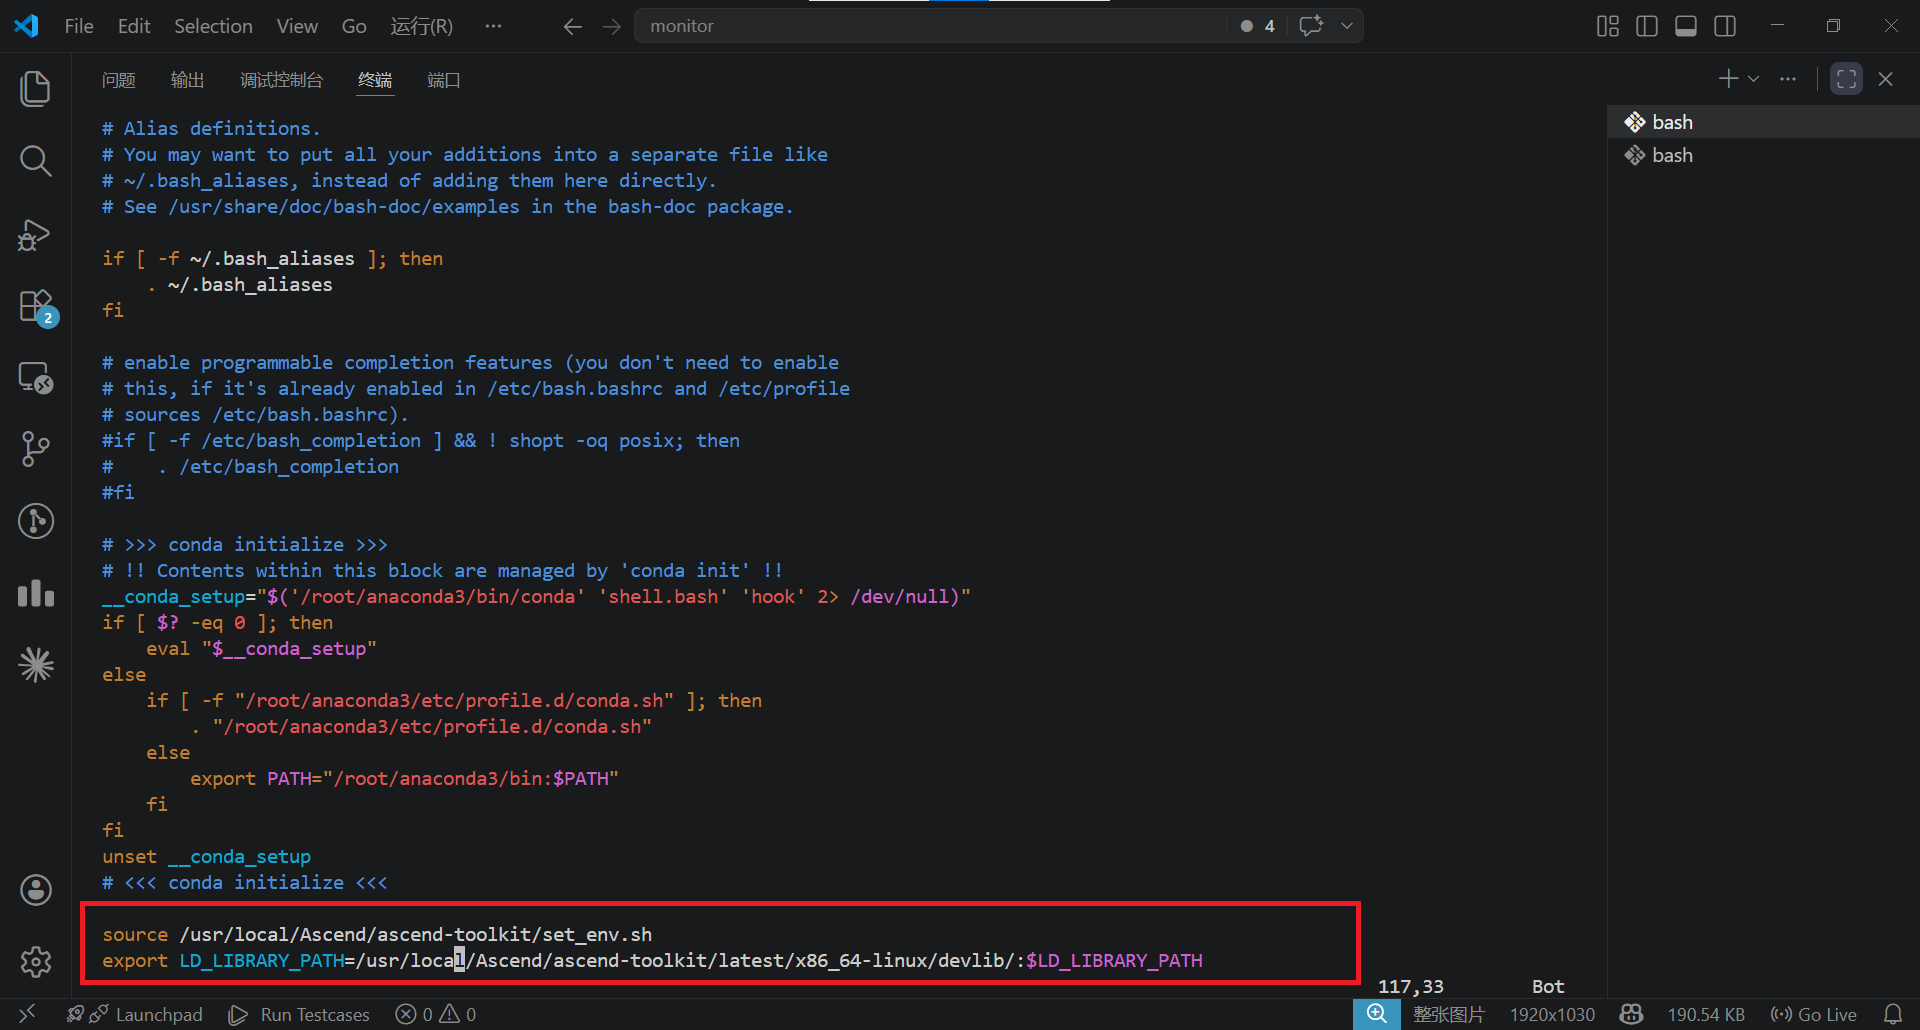
\includegraphics[width=0.8\textwidth]{set-environment.png}
  \caption{环境变量设置}
  \label{fig:set-environment}
\end{figure}
设置完环境变量后，即可在终端输入 atc 命令，验证安装是否成功，此处ATC run failed 是因为没有进入相应的虚拟环境，缺少环境依赖导致的，进入onnx-to-om 虚拟环境后即可恢复正常。
\begin{figure}[H]
  \centering
  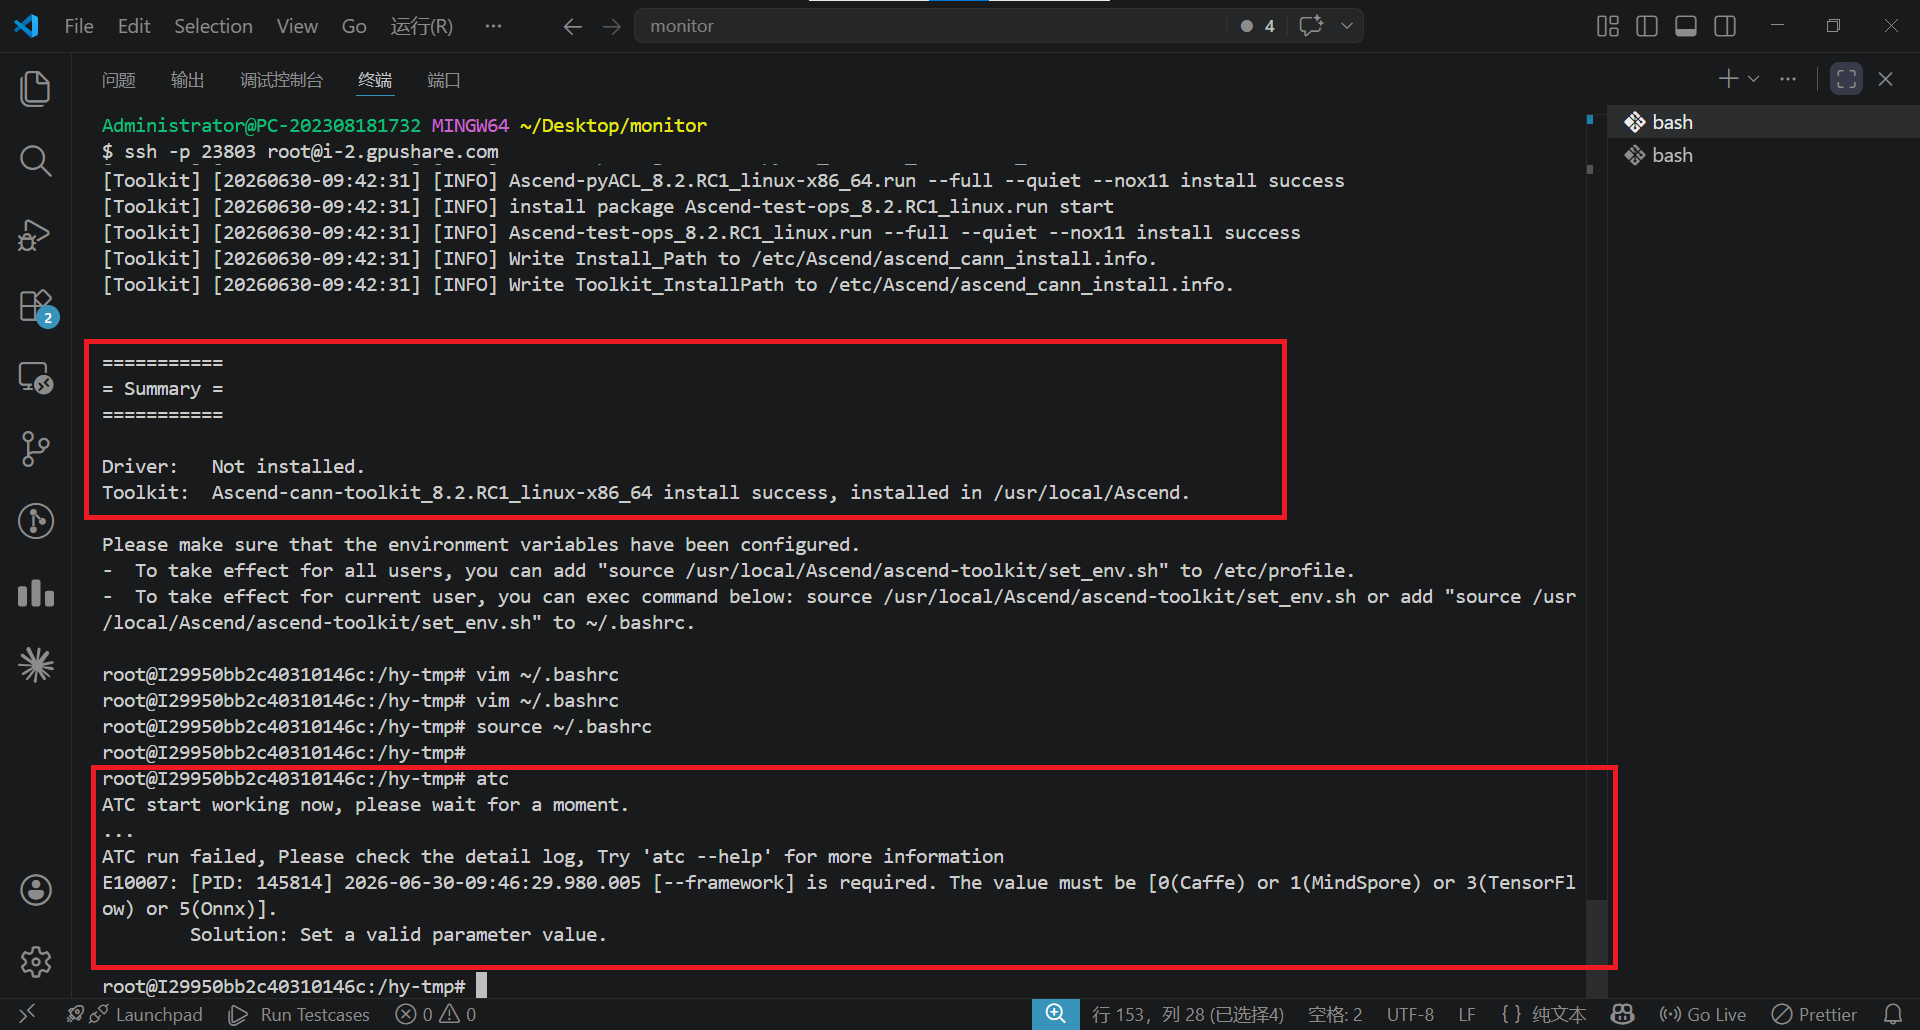
\includegraphics[width=0.8\textwidth]{toolkit-insatll.png}
  \caption{toolkit 安装及测试}
  \label{fig:toolkit-insatll}
\end{figure}

\subsection{模型转换}

将 yolov5s.onnx 放到安装了 Ascend CANN toolkit 的环境中。详细的 ONNX 转 OM 流程可参考\hyperref[ref:onnx2om]{[15]}。

输入以下命令，开始转换，转换时间根据使用机器的性能决定，本组用云服务器转换大概用时1分钟，待输出 ATC run success 表示转换成功，输出如下图所示。
\begin{lstlisting}[style=shell, caption={ONNX 转 OM}]
atc \
  --model=yolov5s.onnx \
  --framework=5 \
  --output=yolov5s_ascend310b \
  --input_format=NCHW \
  --input_shape="images:1,3,640,640" \
  --soc_version=Ascend310B4 \
  --precision_mode=allow_fp32_to_fp16 \
  --log=info
\end{lstlisting}

\begin{figure}[htbp]
  \centering
  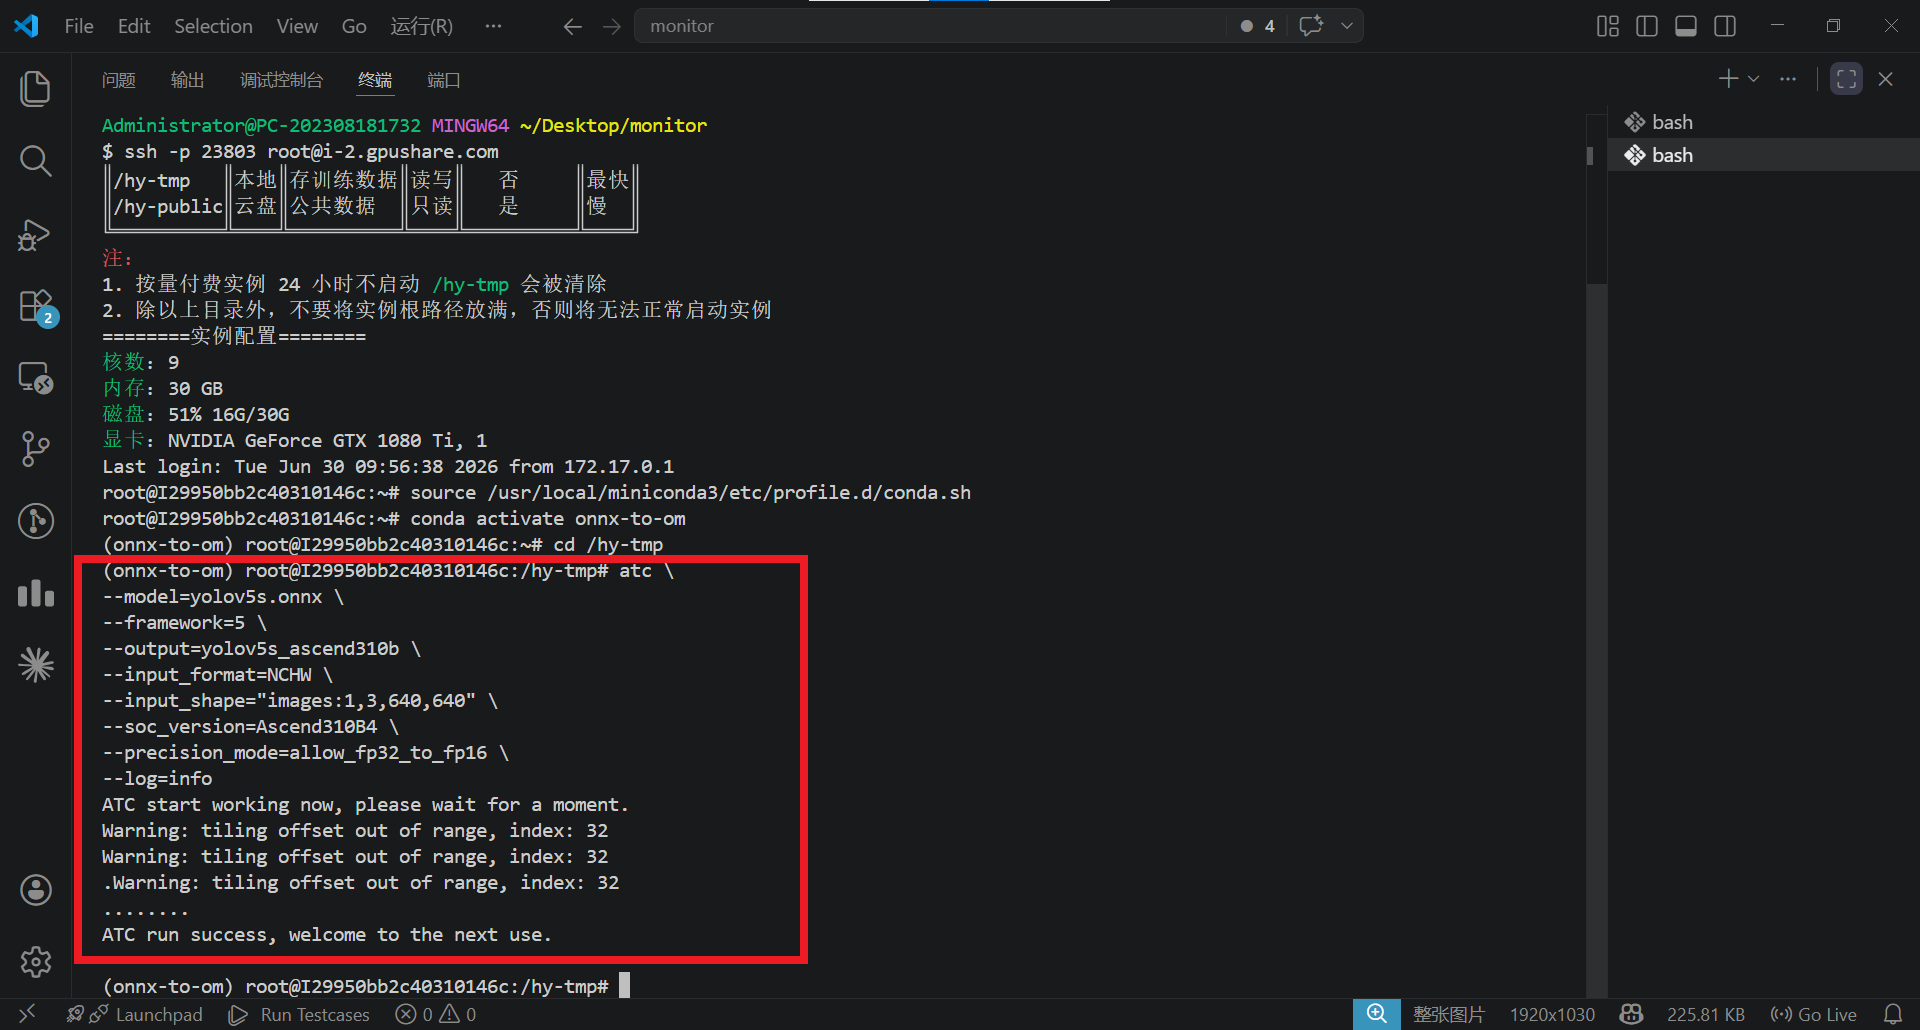
\includegraphics[width=0.8\textwidth]{onnx_to_om.png}
  \caption{模型转换}
  \label{fig:onnx_to_om}
\end{figure}

\section{部署 YOLOv5 CLI 到 OpenHarmony 设备}

在 Windows PowerShell 中进入 \texttt{task3\_yolov5\textbackslash scripts}，执行下面的命令。注意，\texttt{D:\textbackslash models\textbackslash yolov5s\_ascend310b.om} 是 om 模型的位置，\texttt{D:\textbackslash images\textbackslash test.jpg} 是测试图片的位置。

\begin{lstlisting}[style=shell, caption={部署到设备}]
# 不传 Image，使用默认的 example_image\test.jpg
cd scripts
.\hdc_deploy_from_windows.ps1 -LocalProject ..
# 指定自定义图片
.\hdc_deploy_from_windows.ps1 -LocalProject .. -Image D:\images\test.jpg

# 指定模型和图片
.\hdc_deploy_from_windows.ps1 -LocalProject .. -Model D:\models\yolov5s_ascend310b.om -Image D:\images\test.jpg
\end{lstlisting}

部署到设备后目录为：

\begin{lstlisting}[caption={设备端目录结构}]
/cann-install/yolov5_cli/main.py
/cann-install/yolov5_cli/requirements-device.txt
/cann-install/yolov5_cli/scripts/run_on_device.sh
/cann-install/yolov5_cli/models/yolov5s_ascend310b.om
/cann-install/yolov5_cli/images/test.jpg
/cann-install/yolov5_cli/output/
\end{lstlisting}


\section{安装设备端 Python 依赖}

由于任务 2 已经安装过 ais\_bench、aclruntime、numpy、opencv-python，这一步可跳过。


\section{运行 YOLOv5 目标检测}

设备端执行：

\begin{lstlisting}[style=shell, caption={一键运行}]
sh /cann-install/yolov5_cli/scripts/run_on_device.sh
\end{lstlisting}

或手动执行：

\begin{lstlisting}[style=shell, caption={手动运行}]
. /cann-install/task2_cann/03_set_cann_env.sh
cd /cann-install/yolov5_cli
python3.10 main.py \
  --backend ais_bench \
  --device-id 0 \
  --model models/yolov5s_ascend310b.om \
  --image images/test.jpg \
  --output output \
  --img-size 640 \
  --conf-thres 0.25 \
  --iou-thres 0.45 \
  --save-txt \
  --json output/result.json
\end{lstlisting}

输出示例：

\begin{lstlisting}[caption={输出示例}]
[1/1] images/test.jpg -> output/test_detected.jpg, detections=3, latency_ms=18.532
\end{lstlisting}

结果文件：

\begin{lstlisting}[caption={结果文件}]
/cann-install/yolov5_cli/output/test_detected.jpg
/cann-install/yolov5_cli/output/test_detected.txt
/cann-install/yolov5_cli/output/result.json
\end{lstlisting}

拉回 PC：

\begin{lstlisting}[style=shell, caption={拉回结果}]
hdc file recv /cann-install/yolov5_cli/output ./output
\end{lstlisting}

\begin{figure}[htbp]
  \centering
  
\includegraphics[width=0.8\textwidth]{unrecognized.jpg}
  \caption{未识别图片}
  \label{fig:unrecognized}
\end{figure}

\begin{figure}[htbp]
  \centering
  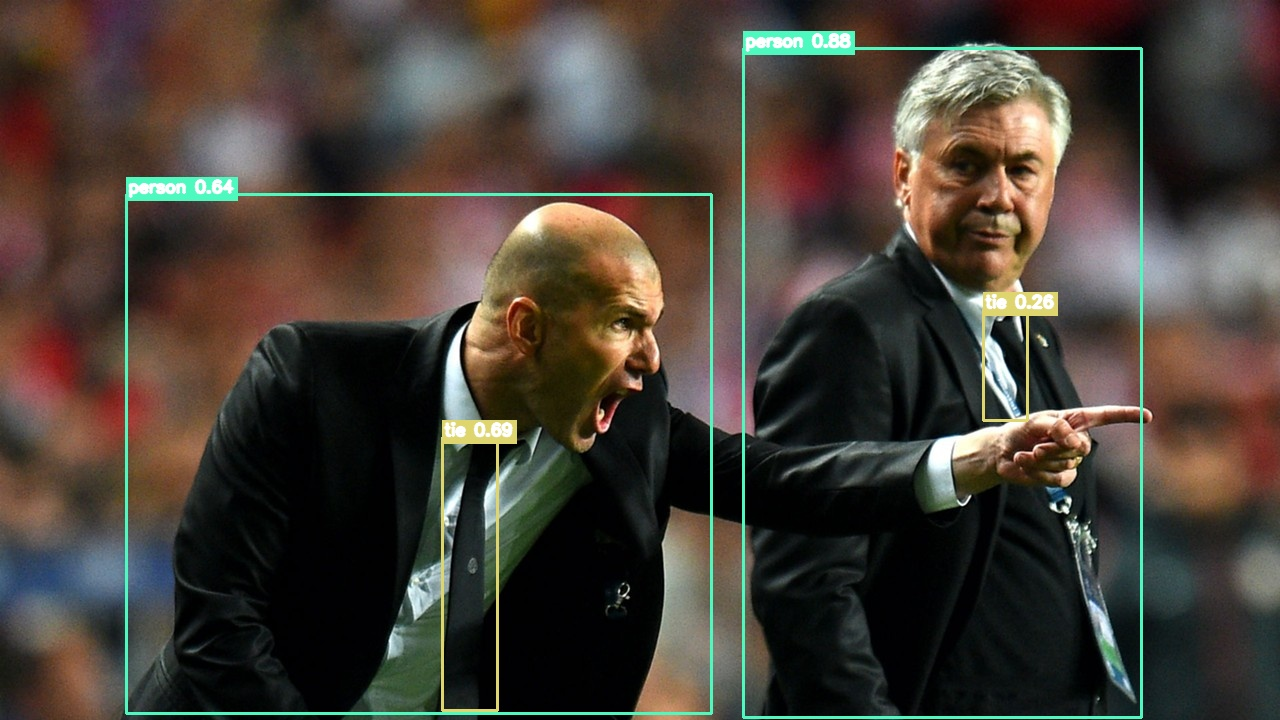
\includegraphics[width=0.8\textwidth]{recognized.jpg}
  \caption{识别结果}
  \label{fig:recognized}
\end{figure}


\section{批量图片推理}

设备端执行：

\begin{lstlisting}[style=shell, caption={批量推理}]
. /cann-install/task2_cann/03_set_cann_env.sh
cd /cann-install/yolov5_cli
python3.10 main.py \
  --backend ais_bench \
  --device-id 0 \
  --model models/yolov5s_ascend310b.om \
  --input-dir images \
  --output output \
  --save-txt \
  --json output/result.json
\end{lstlisting}

程序会递归扫描 images 目录下的 \texttt{.jpg}、\texttt{.jpeg}、\texttt{.png}、\texttt{.bmp}、\texttt{.webp} 文件。


\section{PC 端冒烟测试}

如果想先在 PC 验证 main.py 的前处理、NMS、绘图逻辑，可执行：

\begin{lstlisting}[style=shell, caption={PC 端冒烟测试}]
pip install -r task3_yolov5/requirements/requirements-pc-smoke.txt
python task3_yolov5/server/main.py --backend onnxruntime \
  --model yolov5s.onnx --image test.jpg --output output
\end{lstlisting}

该模式不使用 NPU，只用于本地功能验证。


\section{YOLOv5 CLI 代码结构说明}

main.py 实现了完整的推理流程，如下图所示：

\begin{center}
输入图片 $\rightarrow$ 预处理 $\rightarrow$ NPU 推理 $\rightarrow$ 后处理 $\rightarrow$ 绘制检测框 $\rightarrow$ 保存结果
\end{center}

各函数职责说明：

\begin{itemize}
  \item \texttt{letterbox()}：将输入图片等比例缩放并填充至 $640\times640$，避免目标变形。
  \item \texttt{preprocess()}：将图片从 BGR 格式转为 RGB，调整通道顺序（HWC$\rightarrow$CHW），像素值归一化至 $[0,1]$，生成模型所需的输入张量。
  \item \texttt{InferEngine}：推理引擎封装，根据后端类型自动加载 \texttt{ais\_bench}（NPU）或 \texttt{onnxruntime}（CPU）。
  \item \texttt{postprocess()}：解析模型原始输出，提取检测框坐标和类别置信度，通过 NMS（非极大值抑制）去除重叠框，保留最优结果。
  \item \texttt{draw\_detections()}：在原始图片上绘制检测框和类别标签，生成可视化结果图。
  \item \texttt{save\_txt()}：将检测结果保存为文本文件，每行格式为：类别 ID、置信度、左上角坐标、右下角坐标。
  \item \texttt{-{}-json}：将结构化检测结果和推理耗时保存为 JSON 文件，便于性能分析。
\end{itemize}

默认支持 COCO 数据集的 80 个类别（人、车、狗等）。如需使用自定义类别，可通过 \texttt{-{}-classes} 参数指定类别文件：

\begin{lstlisting}[style=shell, caption={指定自定义类别}]
python3.10 main.py --backend ais_bench --model models/best.om \
  --image images/test.jpg --classes classes.txt --output output
\end{lstlisting}

\noindent 其中 \path{classes.txt} 每行一个类别名称，例如：

\begin{lstlisting}[caption={classes.txt 示例}]
person
car
dog
\end{lstlisting}


\section{输出张量兼容性}

YOLOv5 模型的输出张量包含大量候选检测框，每个框携带位置、置信度和类别信息。本程序支持两种常见的输出格式。

\subsection{标准 YOLOv5 输出}

模型原始输出形状为：

\begin{lstlisting}[caption={标准输出形状}]
[1, 25200, 85]
\end{lstlisting}

\noindent 其含义为：

\begin{itemize}
  \item \textbf{1}：批大小为 1，即一次处理一张图片。
  \item \textbf{25200}：模型在图片上生成了 25200 个候选框。
  \item \textbf{85}：每个候选框包含 85 个数值，具体为：
\end{itemize}

\begin{table}[htbp]
  \centering
  \caption{标准输出每个候选框的 85 个数值含义}
  \label{tab:yolo-output}
  \begin{tabular}{lll}
    \toprule
    字段 & 数量 & 含义 \\
    \midrule
    x, y & 2 & 检测框中心点坐标 \\
    w, h & 2 & 检测框的宽度和高度 \\
    objectness & 1 & 该位置存在目标的置信度（0$\sim$1） \\
    class\_scores & 80 & 80 个类别的得分（COCO 数据集） \\
    \bottomrule
  \end{tabular}
\end{table}

程序通过 \texttt{postprocess()} 对 25200 个候选框进行筛选：先根据置信度阈值过滤低分框，再通过 NMS 去除重叠框，最终保留最优检测结果。

\subsection{包含 NMS 的输出}

部分模型在导出时已内置 NMS 后处理，输出形状为：

\begin{lstlisting}[caption={NMS 后输出形状}]
[N, 6]
\end{lstlisting}

\noindent 其中 N 为最终保留的检测框数量，每个框包含 6 个数值：

\begin{table}[htbp]
  \centering
  \caption{NMS 后输出每个检测框的 6 个数值含义}
  \label{tab:yolo-nms-output}
  \begin{tabular}{lll}
    \toprule
    字段 & 含义 \\
    \midrule
    x1, y1 & 检测框左上角坐标 \\
    x2, y2 & 检测框右下角坐标 \\
    score & 检测置信度 \\
    class\_id & 类别编号 \\
    \bottomrule
  \end{tabular}
\end{table}

本程序可自动识别输出格式并适配处理。


\section{进阶：OpenHarmony 图形应用}

下图为图形应用界面，具体使用流程见演示视频。
\begin{figure}[H]
  \centering
  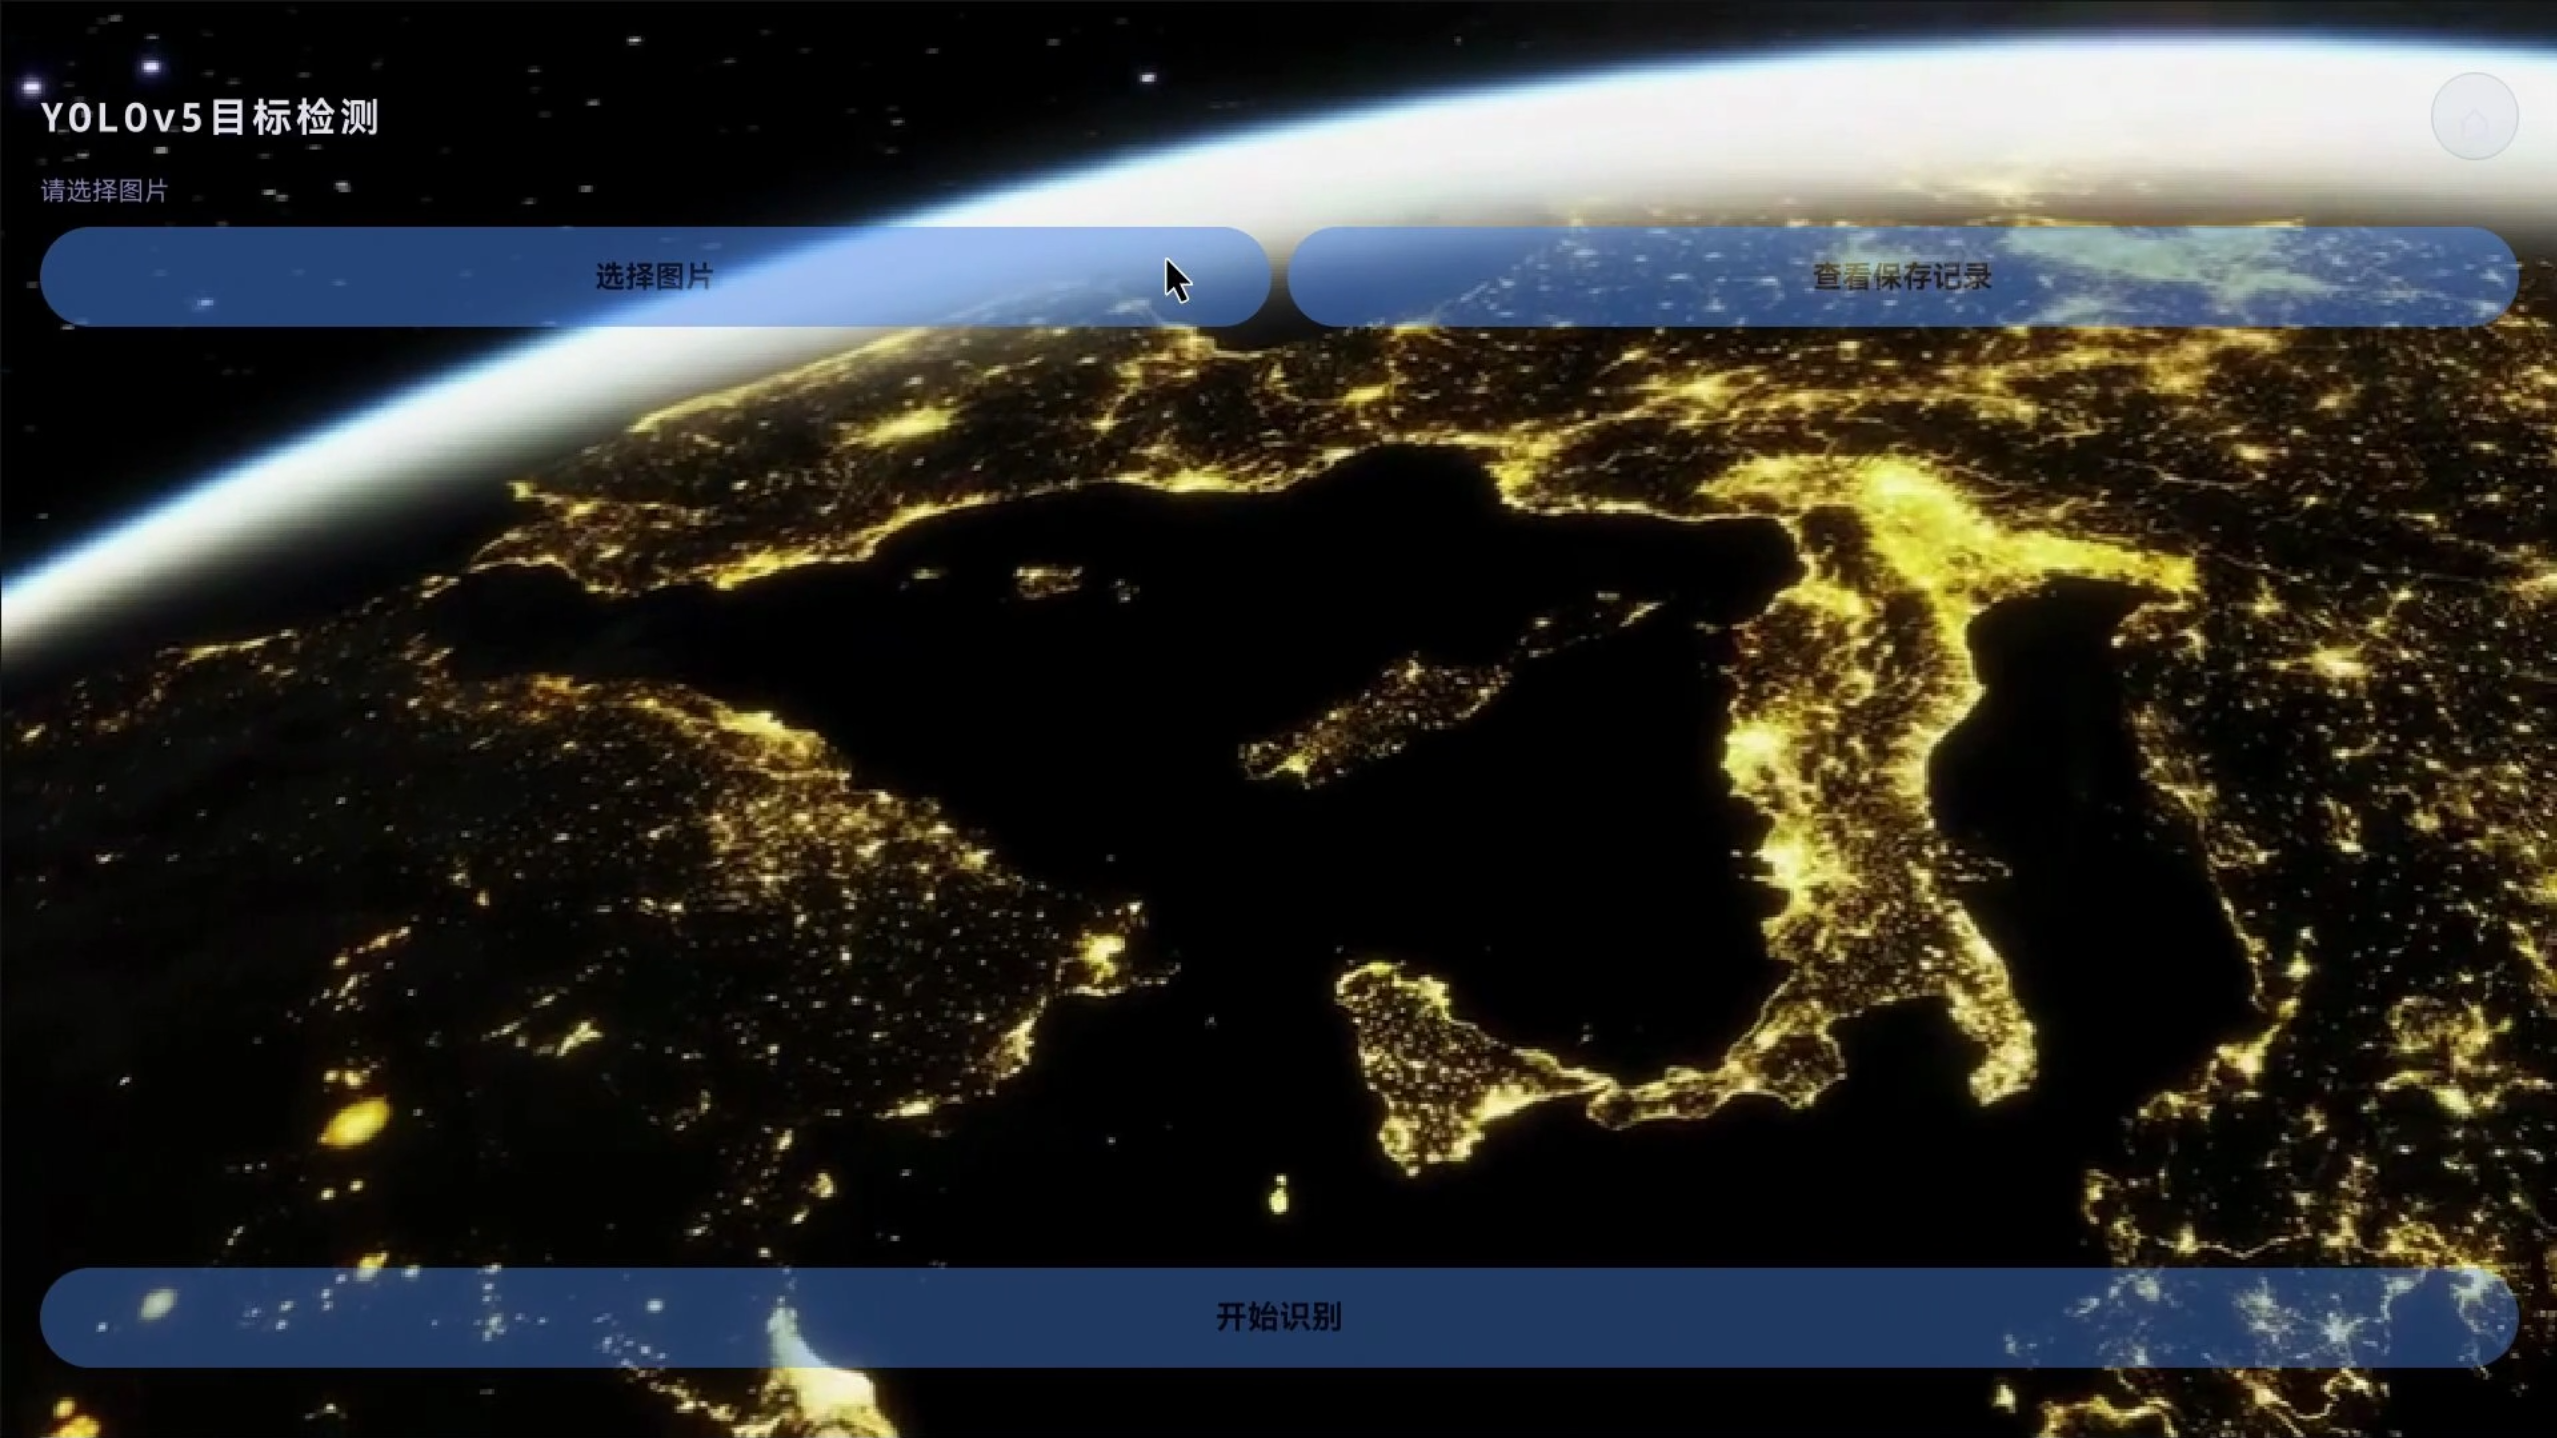
\includegraphics[width=0.8\textwidth]{APP.png}
  \caption{图形应用}
  \label{fig:showapp}
\end{figure}

应用工程中的实时页面位于
\texttt{task3\_yolov5/yolov5\_app/entry/src/main/ets/pages/LiveCamera.ets}，通过
\texttt{libyolo\_napi.so} 调用本机 \texttt{127.0.0.1:5001} 二进制服务；页面本身不调用
Python 或 HTTP。服务端对模型执行持久化加载和 NMS，实时检测优先发送 \texttt{uint8}
NCHW 输入并只返回最多 100 个紧凑检测框。应用同时保留 JPEG 兼容路径，并实现
\texttt{VideoOutput + ImageReceiver + YUV420} 连续分析路径；启动时先检查板端
能力，只有枚举到可用的 YUV420 profile 才启用该路径，否则自动回退到 JPEG。

模型、背景视频和语音提示音已经随工程放在
\texttt{entry/src/main/resources/rawfile/}，不需要从外部网盘补拷。服务启动脚本等待
NPU 节点、CANN 环境和 Python，等待上限为 180 秒；默认 CMake 选项
\texttt{YOLO\_ENABLE\_DIRECT\_ACL=OFF}，禁止在 OpenHarmony musl 应用进程中直接回退
加载 glibc CANN。

\subsection{实时摄像头检测功能说明}

提交 \texttt{3460e25}（feat: YOLOv5 App 新增实时摄像头检测功能及原生 NPU 推理支持）
为图形应用新增实时摄像头检测与原生 NPU 推理能力，主要包含以下新增内容：

\begin{itemize}
  \item 实时摄像头检测页面 \texttt{LiveCamera.ets}：支持摄像头实时预览 +
  NPU 目标检测叠加；
  \item 原生 C++ NPU 推理引擎：
  \begin{itemize}
    \item \texttt{ascend\_cl\_api}：AscendCL 动态加载器（dlopen/dlsym）；
    \item \texttt{yolo\_engine}：YOLO 推理引擎单例（本地 + 远程双模式）；
    \item \texttt{yolo\_napi}：NAPI 绑定（initModel/infer/getModelInfo/releaseModel）；
    \item \texttt{yolo\_live\_napi}：实时帧推理管线（letterbox + NPU 推理 + NMS）；
  \end{itemize}
  \item ArkTS 原生桥接层 \texttt{YoloNativeBridge.ets}；
  \item 设备部署脚本 \texttt{tools/}：CANN 环境配置、ACL 服务自启动；
  \item 技术文档 \texttt{docs/}：Ascend310B YOLOv5 NAPI 集成指南。
\end{itemize}

同时对既有工程做了以下修改：

\begin{itemize}
  \item \texttt{Index.ets}：启动时异步初始化 NAPI 模型，新增
  ``实时摄像头检测''按钮；
  \item \texttt{module.json5}：新增 CAMERA 权限声明；
  \item \texttt{main\_pages.json}：注册 LiveCamera 页面路由；
  \item \texttt{build-profile.json5}：启用 CMake 原生 C++ 构建（arm64-v8a）；
  \item \texttt{oh-package.json5}：声明 libyolo\_napi.so 原生依赖；
  \item \texttt{string.json}：新增摄像头权限说明字符串。
\end{itemize}

\subsection{CANN 运行时随镜像部署与推理服务自启动}

V1.11 将原先依赖 HDC 手工安装的推理环境正式纳入 310B 产品镜像。构建侧把
CANN 8.2.RC1 运行时、Python 3.10、\texttt{numpy}、\texttt{ais\_bench}、
\texttt{aclruntime} 及其依赖打包为
\texttt{/system/var/cann\_runtime\_aarch64.tar.gz}；首次启动由
\texttt{install\_cann\_runtime.sh} 解包到 \texttt{/usr/local}，并使用随包
\texttt{PAYLOAD\_SHA256SUMS} 逐文件校验。安装成功后删除压缩包，后续启动通过
关键文件和清单直接判定环境已就绪，避免重复解压。

设备端服务链路如下：

\begin{lstlisting}[caption={镜像内 CANN 推理服务启动链路}]
post-fs-data
  -> install_cann_runtime.sh
  -> start yolo_acl_service
  -> run_yolo_acl_service.sh
  -> validate Python / ais_bench / numpy / libascendcl.so
  -> wait for three Ascend device nodes (bounded)
  -> listen on 127.0.0.1:5001
\end{lstlisting}

\texttt{init.310B.yolov5.cfg} 将安装和服务启动放在同一个
\texttt{post-fs-data} job 中，服务以 \texttt{HwHiAiUser} 及 NPU 所需补充组运行，
\texttt{once=0} 允许 init 在异常退出后重新拉起。环境脚本固定来自
\texttt{/vendor/etc/yolo\_cann\_env.sh}，不再等待早期教程中的
\texttt{/cann-install/task2\_cann/03\_set\_cann\_env.sh}。启动器对 Python、
\texttt{libascendcl.so}、驱动库和三个 NPU 设备节点分别做有界检查，失败信息写入
\texttt{/data/yolov5\_napi/}，避免无提示无限等待。

应用与服务采用仅绑定 loopback 的二进制协议：NAPI 发送
\texttt{uint8 NCHW} 输入，服务端完成模型持久化、推理和 NMS，只回传最多
100 个检测框。这样不再跨进程传输数百万个浮点输出，也不需要每帧重复加载模型。
OpenHarmony 应用进程使用 musl ABI，而板端 CANN 使用 glibc ABI，因此默认构建项
\texttt{YOLO\_ENABLE\_DIRECT\_ACL=OFF}，明确禁止把 glibc
\texttt{libascendcl.so} 直接加载进应用进程；所有真实 NPU 推理均通过本机服务完成。

应用所需 \texttt{yolov5s\_ascend310b.om}、背景视频及语音提示文件均已放入
\texttt{entry/src/main/resources/rawfile/}，工程不再依赖构建后手工补文件。
